\section{Physikalische Grundlagen}
\label{Kapitel:Rheologie}
In dieser Arbeit werden Flüssigmörtel untersucht, die als kontinuierliches Fluid behandelt werden.
Die dazu notwendigen Gleichungen werden in diesem Kapitel vorgestellt. Diese setzen sich aus den Bilanzgleichungen und deren Schliessungsansätzen zusammen.\\
Zu den Bilanzgleichungen gehören die Erhaltungssätze für Masse und Impuls. Das System ist isotherm, weshalb eine Lösung der Energieerhaltungsgleichung nicht notwendig ist.
Der hochviskose Mörtel ist nahezu inkompressibel und strömt sehr langsam; die Reynoldszahlen liegen im einstelligen Bereich. Es wird deshalb eine konstante Dichte und eine laminare Strömung vorausgesetzt.

Um die Impulsgleichung zu schliessen, ist eine Relation zwischen wirkender Kraft und resultierender Deformation notwendig. Die untersuchten Mörtel besitzen ein sehr komplexes Fliessverhalten, weshalb die Annahme einer Newtonschen Flüssigkeit nicht getroffen werden kann, sondern rheologisch komplexe Gesetze verwendet werden müssen.
%Da die hochviskosen Mörtel nur sehr langsam strömen und die Reynoldszahlen im einstelligen Bereich sind, wird die Strömung als laminar vorausgesetzt.
%In diesem Kapitel werden Gleichungen vorgestellt, die den in dieser Arbeit untersuchten Effekten zugrunde liegen.\\
%Diese bestehen aus den Bilanzgleichungen für inkompressible, isothermische Fluide, die mit rheologischen Stoffgleichungen geschlossen werden.

%Ebenfalls nicht weiter vertieft werden turbulente Eigenschaften und Dichteänderungen, da die Mörtel verhältnismässig langsam strömen und nahezu inkompressibel sind.

%In diesem Kapitel werden die grundlegenden Gleichungen vorgestellt, die in dieser Arbeit benutzt werden.
%Dazu gehören sowohl Erhaltungssätze als auch rheologische Stoffgleichungen.

%Rheologie ist die Wissenschaft über das Verhalten von Stoffen unter Einfluss äusserer Kräfte. Es wird untersucht wie Festkörper, Flüssigkeiten und Gase reagieren wenn sie deformiert werden.
Rheologie ist die Wissenschaft über die Verformung und das Fliessen von Stoffen.
Ein idealer hookscher Festkörper reagiert auf eine Verformung mit einer zur Deformation proportionalen Spannung. Wird keine Kraft mehr auf den Festkörper ausgeübt, führt diese Spannung zu einer Rückkehr zum Anfangszustand. Ein ideales Fluid hingegen setzt einer Verformung zwar einen Widerstand entgegen, baut aber keine Spannung auf. Der Betrag dieses Widerstands ist abhängig von der \glqq{}Flüssigkeit\grqq{} des Fluids, die \linebreak Viskosität genannt wird.\\
In der Realität können viele Materialien nicht in eine der Kategorien Flüssigkeit oder Festkörper eingeteilt werden, weil sie Eigenschaften von beiden besitzen. Die Untersuchung von solchen viskoelastischen Stoffen und ihrem Verhalten unter Einfluss von äusseren Kräften ist einer der Inhalte der Rheologie.
%Dabei wird versucht, die verschiedenen Eigenschaften dieser Stoffe mithilfe von Modellen zu verstehen und nachzubilden.
%, um mit ihnen die Erhaltungssätze zu schliessen.

%
\subsection{Massen- und Impulserhaltung}
Die Massen- und Impulserhaltungsgleichung eines inkompressiblen Fluids können in Matrix-Vektor Form als 
%
\begin{equation}
    \label{eq:Massenerhaltung}
    \nabla \cdot \u = 0
\end{equation}
und
\begin{equation}
    \label{eq:Impulserhaltung}
    \rho \u _t + \rho \u \cdot \nabla\u = -\nabla p +\nabla \cdot \T + \rho \g
\end{equation}
%
geschrieben werden. Dabei ist \nom[gv:u]{$\u$}{Geschwindigkeitsvektor} die Geschwindigkeit, \nom[gv:u]{$p$}{Druck} der Druck, \nom[gv:T]{$\T$}{Spannungstensor} der Spannungstensor, \nom[gv:rho]{$\rho$}{Dichte} die Dichte und $\g$ eine auf das Fluid wirkende, volumetrische Kraft.
Der Einfachheit halber wird im Folgenden angenommen, dass $\g=0$ gilt.\\
Eine ausführliche Herleitung dieser Bilanzgleichungen ist in \cite{boehme} zu finden.

Im allgemeinsten Fall kann der Spannungstensor $\T=f\left( \r,t \right)$\nomenclature[fv:f]{$f$}{Konstitutives Gesetz}\nomenclature[gv:t]{$t$}{Zeit} eine beliebig komplexe Funktion des Ortes und der Zeit sein.
$f$ ist die konstitutive Glei"-chung\footnote{Ein konstitutives Gesetz ist ein Verhältnis zwischen zwei physikalischen Grössen, das Materialspezifisch ist}, die die Spannungen mit den resultierenden Verzerrungen verknüpft.
In dieser Arbeit wird diese Abhängigkeit eingegrenzt, indem $\T$ auf eine Funktion des Dehngeschwindigkeitstensors \nom[gv:D]{$\D$}{Dehngeschwindigkeitstensor} und der Zeit beschränkt wird.
%
\begin{equation}
    \label{eq:Spannungstensor}
    \T = f\left( \D,t \right).
\end{equation}
%
Dabei ist 
\begin{equation}
    \label{eq:Dehngeschwindigkeitstensor}
    \D =\frac{1}{2} \left( \nabla \u + \nabla \u^T \right).
\end{equation}
%
\subsection{Konstitutive Gesetze}
Der Zusammenhang zwischen einer wirkenden Kraft und der resultierenden Dehnung wird durch die Viskosität \nom[gv:eta]{$\eta$}{Viskosität} festgelegt. Diese und andere stoffabhängige Eigenschaften wie die Viskoelastizität werden durch konstitutive Gesetze beschrieben.\\
Die Anforderungen an diese Gesetze sind vielfältig. Einerseits sollen sie die reellen Stoffeigenschaften möglichst gut beschreiben um realitätsnahe Modellierung zu ermöglichen. Andererseits sollen sie die zu lösenden Glei"-chungen nicht unnötig komplizieren und deshalb mit einfachen Zusammenhängen und wenig Parametern auskommen.\\
Aus diesen Anforderungen ist eine Vielzahl von Modellen für Fliessgesetze entstanden, von denen einige nachfolgend aufgeführt werden. Weitere Modelle werden in \cite{boehme}, \cite{introtorheo} und \cite{comprheo} beschrieben.

\subsubsection{Zeitunabhängige Spannungen}
Ist $\T$ keine Funktion der Zeit, gilt $\T=f\left( \D \right)$.
Ein Spezialfall dieses Modells ist die Newtonsche Flüssigkeit, für die $\T=2\eta\D$ gilt. In diesem Fall wird oft auch die Variable \nom[pv:mu]{$\mu$}{Konstante Viskosität eines newtonschen Fluides} statt $\eta$ verwendet.

Statt $\T=f\left( \D \right)$ wird oft auch der Ausdruck
\begin{equation}
    \label{eq:TgeneralNewton}
    \T=\eta\left( \D \right)\cdot \D
\end{equation}
verwendet. Diese Darstellung ermöglicht es, von einem generalisiertem Newtonschen Fluid zu sprechen, bei dem die effektive Viskosität $\eta$ abhängig von der Dehngeschwindigkeit $\D$ ist.

Wird angenommen, dass $\eta$ nur von der Summe aller Dehngeschwindigkeiten abhängt (isotrope Viskosität), kann man $\D$ mit der Scherrate \nom[gv:gamma]{$\gammap$}{Scherrate} ersetzen:
\begin{equation}
    \label{eq:Scherrate}
    \gammap := \sqrt{2 \cdot \D\dipr\D},
\end{equation}
wobei
\begin{equation}
    \label{eq:doubleInnerProduct}
    \A\dipr\B := \sum_{i,j}{a_{ij}b_{ij}}
\end{equation}
das doppelte innere Produkt ist.

Die Funktion $\eta\left( \gammap \right)$ wird auch Fliesskurve genannt. Sie beschreibt die Änderung der Viskosität von Fluiden bei einer Scherung.\\
Dabei kann man die Fluide in verschiedene Kategorien unterteilen. Dilatante Fluide werden zähflüssiger, wenn sie geschert werden; strukturviskose Fluide haben eine sinkende Viskosität für steigende Scherraten.
Ein Spezialfall der Strukturviskosität ist die Viskoplastizität, bei der erst nach dem Überschreiten einer Fliessgrenze ein Fliessvorgang möglich ist. Unterhalb dieser Grenze verhält sich ein viskoplastisches Material wie ein Fest"-körper.\\
In Abbildung~\ref{fig:fliessKurven} sind die Fliesskurven der verschiedenen Fluid-Typen dar\-ge\-stellt. Im Folgenden werden einige Modelle für Fliessfunktionen vorgestellt. 
%
%Mit Hilfe von \eqref{eq:Scherrate} lassen sich diese in zwei Kategorien unterteilen. Dilatante Fluide werden zähflüssiger wenn sie geschert werden, strukturviskose Fluide haben eine sinkende Viskosität für steigende Scherraten. 
%Die konstante Viskosität eines Newtonschen Fluids kann ebenfalls als Fliessfunktion geschrieben werden, wobei $\eta\left( \gammap \right)=\mu$.
%Ein Spezialfall des strukturviskosen Fluids ist die Viskoplastizität, bei der erst nach dem Überschreiten einer Fliessgrenze ein Fliessvorgang möglich ist. Unterhalb dieser Grenze verhält sich ein viskoplastisches Material wie ein Festkörper.\\
%In Abbildung~\ref{fig:fliessKurven} einige dieser Fliesskurven dargestellt.
%
\begin{figure}
    \centering
    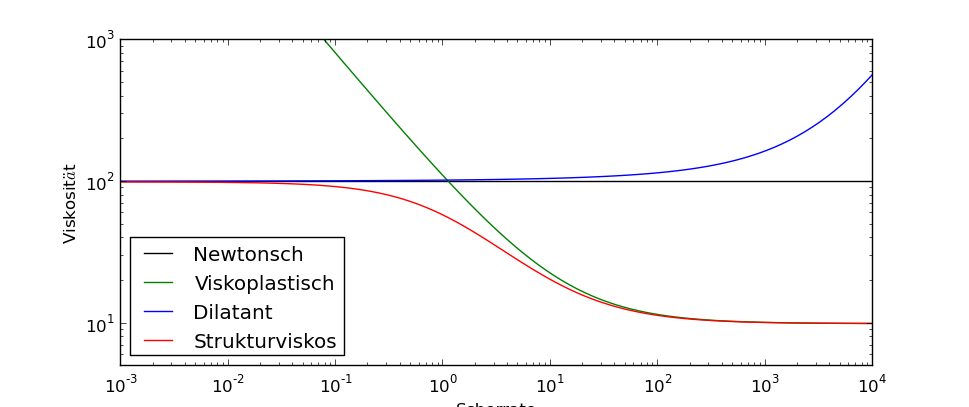
\includegraphics[width=\textwidth]{figures/Fliesskurven.png}
    \caption{Fliesskurven von verschiedenen Typen von Fluiden, dargestellt im doppelt logarithmischen Plot}
    \label{fig:fliessKurven}
\end{figure}
%
%\begin{table}
    %\centering
    %\begin{tabular}{l l l}
        %Modell & Fliessfunktion & Parameter \\
        %\hline
        %Newton & $\mu= \mbox{const}$ & $\mu$ \\ 
        %Ostwald-de Waele & $\eta=K \gammap^{n-1}$ & $K,n$ \\ 
        %Bingham-Modell & $\eta= \frac{\tau_0}{\gammap}+K $ & $\tau_0,K$ \\ 
        %Carreau-Yasuda & $\eta=\eta_\infty+\left( \eta_0-\eta_\infty \right)\left[ \left( \gammap \right)^\alpha \right] ^{\frac{n-1}{\alpha}} $ & $\eta_0,\eta_\infty,\alpha,n$ \\ 
        %Herschel-Bulkley & $\eta= \frac{\tau_0}{\gammap}+K\gammap^{n-1} $ & $\tau_0,K,n$
    %\end{tabular}
    %\caption{Fliessgesetze für zeitunabhängige Spannungen}
    %\label{tab:Fliessgesetze}
%\end{table}
%
\paragraph{Empirische Fliessgesetze}~\\*~\\*
Eine Approximation der Fliesskurven durch analytische Funktionen er\-mög\-licht eine geschlossene Behandlung der Gleichungen, ohne dass auf Tabellendaten oder andere Hilfsmittel zurückgegriffen werden muss.\\
Solche Modelle enthalten eine bestimme Anzahl freier Parameter, die an das jeweilige Material angepasst werden müssen.
\subparagraph{Newton}
Das Newtonsche Fliessgesetz kann ebenfalls als analytisches Modell mit dem Parameter $\mu$ aufgefasst werden.
\begin{equation}
    \eta = \mu.
    \label{eq:fg:newton}
\end{equation}
\subparagraph{Ostwald-de-Waele}
Das einfachste nicht-Newtonsche Fliessgesetz ist das Potenzgesetz nach Ostwald und de~Waele,
\begin{equation}
    \eta=K\gammap^{n-1}.
    \label{eq:fg:potenz}
\end{equation}
Es besitzt zwei Parameter, den Fliessindex \nom[pv:n]{$n$}{Fliessindex in Fliessgesetzen} und den Konsistenzparameter \nom[pv:K]{$K$}{Konsistenzparameter in Fliessgesetzen}. Der Fliessindex entscheidet dabei über das Verhalten des Fluids bei sich ändernder Scherrate (Dilatant für $n>1$, Struktuviskos für $n<1$ oder Newtonsch für $n=1$), der Konsistenzparameter ähnelt der Viskosität bei newtonschen Flüssigkeiten.
%
\subparagraph{Carreau-Yasuda}
Ein Mangel des Ostwald-de-Waele-Modells ist das unrealistische Verhalten beim Grenzübergang $\gammap\rightarrow 0$. Abhängig von $n$ geht die Viskosität gegen Unendlich oder gegen Null.
Eine Möglichkeit dies zu beheben, bietet das Carreau-Yasuda-Modell,
\begin{equation}
    \eta=\eta_\infty+\left( \eta_0-\eta_\infty \right)\left[ 1+\left( L\gammap \right)^\alpha \right] ^{\frac{n-1}{\alpha}},
    \label{eq:fg:carreauyasuda}
\end{equation}
durch den Parameter \nom[pv:xc:eta0]{$\eta_0$}{Nullviskosität im Carreau-Yasuda Modell}, der das Grenzverhalten für $\gammap\rightarrow0$ steuert. Desweiteren beinhaltet das Modell eine Grenzviskosität \nom[pv:xc:etainf]{$\eta_\infty$}{Grenzviskosität im Carreau-Yassuda Modell}, die Zeitkonstante \nom[pv:xc:L]{$L$}{Zeitkonstante im Carreau-Yasuda Modell}, der Fliessindex $n$ und den Parameter \nom[pv:xc:alpha]{$\alpha$}{Parameter im Carreau-Yasuda Modell}, der den Übergang zwischen Null- und Grenzviskosität steuert.
%
\subparagraph{Bingham}
Ein Bingham Fluid ist ein Material, der erst ab einer Fliessgrenze zu fliessen beginnt, danach aber Newtonsches Verhalten zeigt.
\begin{equation}
    \eta=
    \begin{cases}
        \infty                           & \tau<\tau_{0}    \quad \text{(Festkörper)}\\
        \frac{\tau-\tau_{0}}{\mu\cdot\gammap} & \tau\geq\tau_{0}
    \end{cases}
    \label{eq:fg:bingham}
\end{equation}
Dabei ist \nom[pv:xb:tau0]{$\tau_0$}{Fliessgrenze von viskoplastischen Materialien} die Fliessgrenze und $\mu$ die Viskosität im Newtonschen Bereich.
%
\subparagraph{Herschel-Bulkley Modell}
Ein Modell mit einer Fliessgrenze und einem nicht-Newtonschen Verhalten oberhalb dieser Grenze ist das Herschel"=Bulkley"=Modell.
\begin{equation}
    \eta=  \frac{\tau_0}{\gammap}+K\gammap^{n-1}.
    \label{eq:fg:herschelbulkley}
\end{equation}
%Die Parameter sind die Fliessgrenze $\tau_0$ und der Konsistenzparameter $K$.

Die scherratenabhängige Viskosität einiger von Hilti hergestellten Mörteln wurde schon in früheren Arbeiten untersucht.\todo{Marco zitieren}
Die Mörtel zeigen ein viskoplastisches Verhalten, das sich am besten mit dem modifizierten Herschel-Bulkley Modell abbilden lässt:
\begin{equation}
    \label{eq:modHB}
    \eta\left( \gammap \right) = \tau_0 \frac{1-\exp \left( -m\gammap \right)}{\gammap}+K\gammap^{n-1}.
\end{equation}
Die materialabhängigen Parameter sind dabei die Fliessgrenze $\tau_0$, die Konsistenz $K$ und der Fliessindex $n$. Der Parameter $m$ bestimmt das Verhalten des Modells bei sehr kleinen Scherraten und wurde in der vorliegenden Arbeit auf 1000 gesetzt.%Im Bild [\ref{fig:modHBKurven}] \todo{Bild} ist der Zusammenhang zwischen Viskosität und Scherrate für verschiedene Parametersets aufgetragen.
%In Tabelle \ref{tab:Fliessgesetze} sind weitere dieser Fliessgesetze genannten Modelle aufgeführt.
%
\subsubsection{Zeitabhängige Spannungen}
Für viele Flüssigkeiten spielt nicht nur der aktuelle Zustand des Fluids eine Rolle, sondern auch die Geschichte der früheren Deformationen. Die konstitutive Gleichung $f$ ist also nicht mehr nur von $\D$ abhängig, sondern auch von der Zeit $t$ und der Verzerrungsgeschichte:
\begin{equation}
    \label{eq:Tviskoelastisch}
    \T\left( \D,t \right) = \underset{s\leq t}{f}\left[ \T\left( s \right),\D\left( t \right) \right].
\end{equation}

\paragraph{Maxwell Modell}
Ein Modell um das Verhalten solch eines Stoffes zu be"-schrei"-ben, ist das Maxwell Modell.
Dabei wird das Material als eine Mischung aus einer viskosen Newtonschen Flüssigkeit und einem oder mehreren elastischen Festkörper beschrieben. Das geschieht durch eine Kombination aus einem Dämpfer und einer Feder, deren Eigenschaften in Reihe geschalten sind. 
Eine schematische Darstellung ist in Abbildung~\ref{fig:Maxwell-Material} zu sehen.\\
Wird nun auf dieses Material eine Kraft in Form einer Spannung ausgeübt, nehmen beide Komponenten einen Teil davon auf, wobei der viskose Dämp"-fer sich unter der Spannung verformt und die Energie als Wärme dissipiert. Die elastische Komponente speichert die Spannung hingegen als elastische Energie und kann diese zu einem späteren Zeitpunkt wieder zurückgeben.
%
\begin{figure}
    \centering
    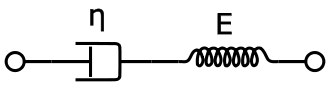
\includegraphics[width=0.5\textwidth]{figures/Maxwell-material.png}
    \caption{Schematische Darstellung des Maxwell - Materials.\\
    Links der viskose Dämpfer, rechts die elastische Feder.}
    \label{fig:Maxwell-Material}
\end{figure}

Die resultierende Differentialgleichung für die Schubspannung $\T$ nimmt folgende Form an:
%
\begin{equation}
    \label{eq:maxwellModell}
    \T + \lambda \frac{\partial\T}{\partial t}=2\eta \D.
\end{equation}
Die Voraussetzung dafür ist, dass das Stoffverhalten als linear angenommen wird. Das bedeutet es werden nur Verzerrungen mit hinreichend kleiner Amplitude betrachtet. Zusätzlich muss noch die Annahme eines exponentiell schwindenden Gedächtnisses getroffen werden. Das heisst der Einfluss von Verzerrungen auf die aktuelle Spannung nimmt mit der Zeit exponentiell ab.
Wie schnell dieser Einfluss abnimmt, hängt dabei von der Relaxationszeit \nom[gv:lambda]{$\lambda$}{Relaxationszeit eines viskoelastischen Materials} ab.

\paragraph{Oldroyd-B Modell}
Eine Erweiterung des Maxwell Modells ist das Oldroyd"~B Modell, bei dem statt der partiellen die kontravariante Ableitung \nom[not:oldroyd]{$\overset{\nabla}{\T}$}{Oldroydsche Zeitableitung} verwendet wird:
\begin{equation}
    \label{eq:oldroydModell}
    \T + \lambda \overset{\nabla}{\T}=2\eta \D
\end{equation}
wobei
\begin{equation}
    \label{eq:upperconvectedDerivative}
    \overset{\nabla}{\T} = \frac{D}{Dt}\T-\left[ \nabla \u^T\cdot \T \right]-\left[ \T\cdot \nabla \u \right].
\end{equation}
Diese Modifikation dient dazu, Drehungen und Verzerrungen des Fluides in der Differentialgleichung zu berücksichtigen.
Die Herleitung dieser Ab"-lei"-tung stammt von J.G. Oldroyd \cite{oldroyd}, nach dem auch das Modell benannt ist.

\paragraph{White-Metzner Modell}
Das in dieser Arbeit verwendete Modell für visko"-elastische Fluide muss zusätzlich zu der Zeitabhängigkeit auch die stark Scherratenabhängigkeit berücksichtigen können.\\
Dazu in der Lage ist das White-Metzner Modell. Dieses ist eine Erweiterung des Oldroyd-B Modelles, bei dem zusätzlich $\lambda$ und $\eta$ eine Funktion von $\gammap$ sind:
\begin{equation}
    \label{eq:whiteMetznerModell}
    \T + \lambda\left( \gammap \right) \overset{\nabla}{\T}=2\eta\left( \gammap \right) \D.
\end{equation}
Dabei können im Allgemeinen für die Funktionen $\lambda$ und $\eta$ die selben Modelle wie für die nicht zeitabhängigen Gesetze verwendet werden.
In dieser Arbeit wurde für $\eta$ das schon bewährte modifizierte Herschel-Bulkley Modell \eqref{eq:modHB} implementiert.\\
Die Relaxationszeit weist für die untersuchten Mörtel, abhängig von der Scherrate, zwei Plateaus auf; bei einer hinreichend kleiner und grosser Scherrate. Dazwischen verläuft der Übergang exponentiell, wie in Abbildung~\ref{fig:carreauYasudaAnnotated} gezeigt.
Als beschreibende Funktion für $\lambda$ wird daher auf Emp\-feh\-lung des Rheologiespezialisten von Hilti das Carreau-Yasuda Modell \eqref{eq:fg:carreauyasuda} verwendet.
%
\begin{figure}[h]
    \centering
    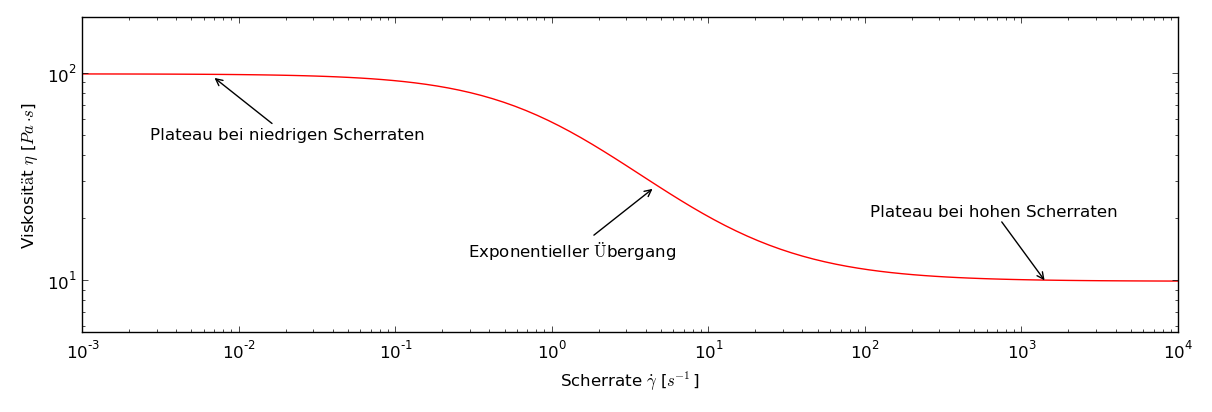
\includegraphics[width=\textwidth]{figures/CarreauYasudaAnnotated.png}
    \caption{Beispielkurve des Carreau-Yasuda Modells.}
    \label{fig:carreauYasudaAnnotated}
\end{figure}
%\begin{equation}
    %\label{eq:carreauYasuda}
    %\lambda \left( \gammap \right) = \eta_{\infty} +\left( \eta_0 - \eta_{\infty} \right) \left( 1+\left( L\gammap \right)^\alpha \right)^{\frac{n_{\lambda}-1}{\alpha}}.
%\end{equation}
%
%Die Parameter $\eta_{\infty}$, $\eta_0$, $L$, $\alpha$ und $n_{\lambda}$ sind dabei wieder materialabhängig. 
%
%\subsubsection{Strukturviskosität}
%%
%\subsubsection{Viskoelastizität}
%%
%\subsubsection{Konstitutive Gesetze}
